\section{Results}

All values are medians of the measured samples; values in parentheses are IQRs. Times are \emph{per
multiplication}, kernel only (Section~\ref{sec:timer}). The raw samples (including warm-up) are in
\texttt{results/raw\_measurements.csv}; per-run information is in \texttt{results/runs.csv}.

\subsection{Correctness}
All $52$ checks of the pre-benchmark test script passed (Table~\ref{tab:correct}); the maximum observed relative
error against NumPy was $7.6\times10^{-16}$ ($n=100$), far below the a-priori bound. In the benchmark, all
\textbf{92 completed runs} (43 of the main campaign and 49 supplementary) passed the element-wise check and the checksum
check (largest relative error $8.3\times10^{-15}$, i.e.\ below $10\,\%$ of the accepted bound; per-run values in
\texttt{runs.csv}), and the final $C$ of C, Java and Python was \textbf{bit-for-bit identical} for every size where
more than one language completed (SHA-256 of the dumped matrix, \texttt{results/summary\_bitwise.csv}). The
identical bits are expected because all three programs use the same operation order, binary64 arithmetic and no
fused multiply--add.

\begin{table}[H]
\centering\footnotesize
\begin{tabular}{llrrl}
\toprule
Test (all three languages) & Check & Max. rel./abs. error & Tolerance & Result \\
\midrule
scalar 1x1 (3*4) & exact & 0 & 0 (exact) & pass \\
hand-computed 3x3 & exact & 0 & 0 (exact) & pass \\
2x2 non-commutative & exact & 0 & 0 (exact) & pass \\
zero * random (n=7) & exact & 0 & 0 (exact) & pass \\
identity * B (n=16) & exact & 0 & 0 (exact) & pass \\
A * identity (n=16) & exact & 0 & 0 (exact) & pass \\
all-ones (n=32) $\rightarrow$ every entry 32 & exact & 0 & 0 (exact) & pass \\
random integers 0..99 (n=64), exact & exact & 0 & 0 (exact) & pass \\
random [0,1) n=5 vs NumPy & tol & 1.8e-16 & 1.1e-15 & pass \\
random [0,1) n=17 vs NumPy & tol & 2.2e-16 & 3.8e-15 & pass \\
random [0,1) n=33 vs NumPy & tol & 5.6e-16 & 7.3e-15 & pass \\
random [0,1) n=64 vs NumPy & tol & 4.3e-16 & 1.4e-14 & pass \\
random [0,1) n=100 vs NumPy & tol & 7.6e-16 & 2.2e-14 & pass \\
\bottomrule
\end{tabular}

\caption{Pre-benchmark correctness tests (each run in C, Java and Python; bit-for-bit identical across languages in every test).}
\label{tab:correct}
\end{table}

\subsection{Runtime versus matrix size}
Table~\ref{tab:time} and Figure~\ref{fig:time} show the runtime. For small sizes the values come from batches
(Section~\ref{sec:timer}); at the largest sizes only 2--3 repetitions were affordable. At $n\ge 1500$ Python hit
the 300\,s limit and from $n=3000$ Java did (Table~\ref{tab:limits}).

\begin{table}[H]
\centering\footnotesize
\setlength{\tabcolsep}{4pt}
\begin{tabular}{rllll}
\toprule
$n$ & C & Java & Python & reps (C/J/P) \\
\midrule
10 & 0.526\,$\mu$s (0.0102\,$\mu$s) & 0.949\,$\mu$s (0.168\,$\mu$s) & 57.5\,$\mu$s (7.37\,$\mu$s) & 10/10/10 \\
50 & 95.7\,$\mu$s (3.25\,$\mu$s) & 119\,$\mu$s (23.4\,$\mu$s) & 7.13\,ms (604\,$\mu$s) & 10/10/10 \\
100 & 816\,$\mu$s (38.8\,$\mu$s) & 990\,$\mu$s (83.6\,$\mu$s) & 50.1\,ms (3.56\,ms) & 10/10/10 \\
200 & 8.39\,ms (261\,$\mu$s) & 9.12\,ms (112\,$\mu$s) & 487\,ms (52.8\,ms) & 10/10/10 \\
256 & 19.8\,ms (1.36\,ms) & 19.9\,ms (2.91\,ms) & 1.07\,s (91.4\,ms) & 10/10/5 \\
400 & 81.1\,ms (10.4\,ms) & 100\,ms (7.84\,ms) & 5.25\,s (165\,ms) & 10/10/5 \\
500 & 154\,ms (5.88\,ms) & 198\,ms (10.3\,ms) & 11.4\,s (93.9\,ms) & 10/10/5 \\
512 & 284\,ms (39.7\,ms) & 219\,ms (23.6\,ms) & 12.8\,s (260\,ms) & 10/10/5 \\
800 & 700\,ms (11.8\,ms) & 831\,ms (76.9\,ms) & 46.3\,s (920\,ms) & 5/5/3 \\
1000 & 1.33\,s (30.6\,ms) & 2.02\,s (118\,ms) & 98.9\,s (1.79\,s) & 5/5/3 \\
1024 & 3.34\,s (196\,ms) & 3.21\,s (94.8\,ms) & 107\,s (1.16\,s) & 5/5/2 \\
1250 & 4.33\,s (1.55\,s) & 10.2\,s (201\,ms) & 207\,s (940\,ms) & 5/5/2 \\
1500 & 6.46\,s (332\,ms) & 28\,s (321\,ms) & \textit{timeout} & 5/5/-- \\
2000 & 33.4\,s (600\,ms) & 86.9\,s (494\,ms) & \textit{not attempted} & 5/3/-- \\
2048 & 44.2\,s (2.89\,s) & 95\,s (541\,ms) & \textit{not attempted} & 3/2/-- \\
3000 & 185\,s (981\,ms) & \textit{timeout} & \textit{not attempted} & 2/--/-- \\
\bottomrule
\end{tabular}

\caption{Median (IQR) time of one multiplication, and number of measured repetitions per implementation. Italics: no
time exists for that configuration (timeout at the $300$\,s per-sample limit, or not attempted because an earlier size already failed).}
\label{tab:time}
\end{table}

\begin{figure}[h]
\centering
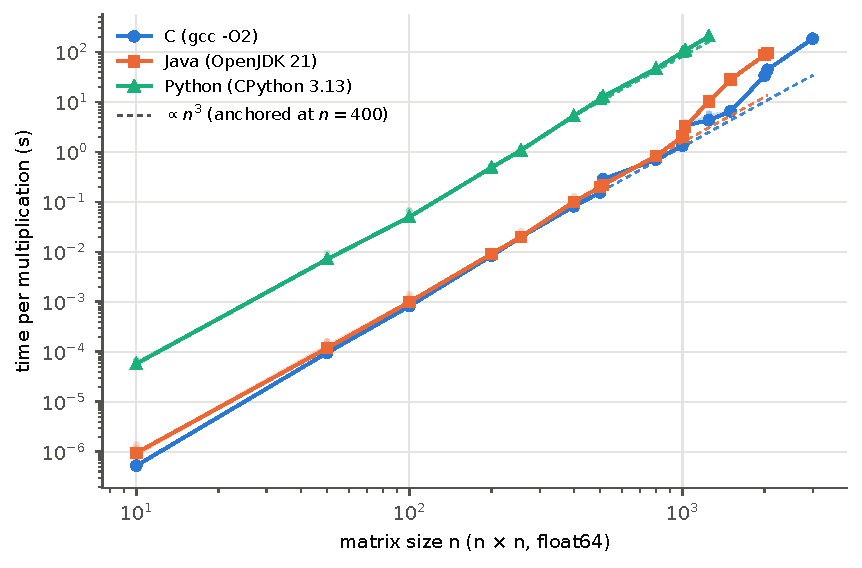
\includegraphics[width=0.86\linewidth]{../figures/fig1_runtime_loglog.pdf}
\caption{Median time per multiplication against $n$ (log--log). Bands: IQR; faint points: individual repetitions;
dashed lines: $n^3$ growth anchored at $n=400$. Python was run only up to $n=1250$ and Java up to $n=2048$ within the budget.}
\label{fig:time}
\end{figure}

\paragraph{Growth.} A least-squares fit of $\log t$ against $\log n$ gives exponents close to the cubic model only
for small to medium sizes (Table~\ref{tab:fit}): $3.17$--$3.27$ for $50\le n\le400$ in all three languages. Over the
larger windows the exponent is $3.29$ for Python, $3.63$ for C and $4.01$ for Java, i.e.\ the cost per multiply--add
is not constant. Figure~\ref{fig:norm} shows this directly: the time per multiply--add $t/n^3$ is almost flat for
Python and for C/Java up to $n\approx 1000$, and then grows (C: $1.3\to6.8$\,ns, Java: $2.0\to11.1$\,ns).
At $n=512$ and $n=1024$ C has isolated spikes (Section~\ref{sec:pow2}).

\begin{table}[H]
\centering\small
\begin{tabular}{llrrl}
\toprule
Impl. & Sizes used ($n$) & Points & Exponent $k$ & 95\,\% CI \\
\midrule
C & 50--400 & 5 & 3.27 & [3.16, 3.38] \\
C & 200--3000 & 13 & 3.63 & [3.37, 3.89] \\
Java & 50--400 & 5 & 3.22 & [3.04, 3.40] \\
Java & 200--2048 & 12 & 4.01 & [3.67, 4.36] \\
Python & 50--400 & 5 & 3.17 & [2.92, 3.43] \\
Python & 200--1250 & 9 & 3.29 & [3.19, 3.39] \\
\bottomrule
\end{tabular}

\caption{Empirical exponent $k$ in $t\propto n^{k}$ (least squares on the medians, 95\,\% $t$-interval). The interval reflects the scatter of the medians around the line, not between-process variability (Section~\ref{sec:procvar}).}
\label{tab:fit}
\end{table}

\begin{figure}[h]
\centering
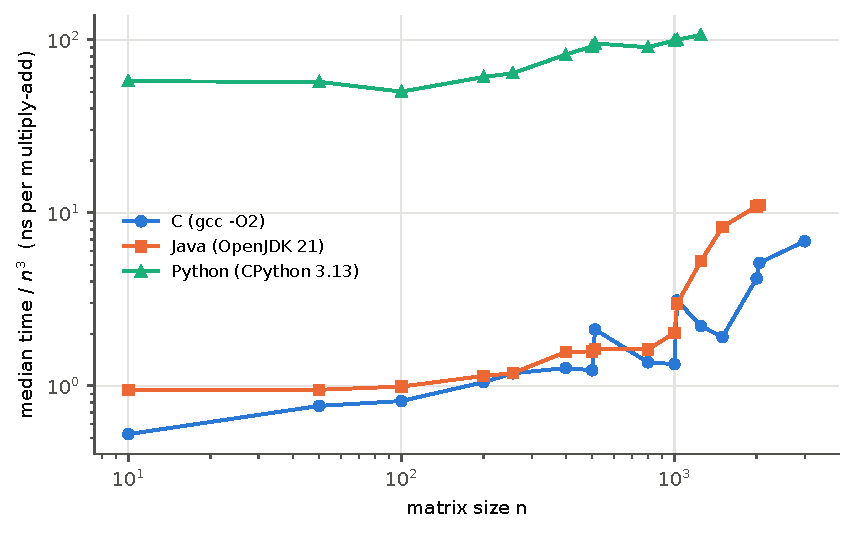
\includegraphics[width=0.82\linewidth]{../figures/fig2_normalised_time.pdf}
\caption{Median time divided by $n^3$ (nanoseconds per multiply--add). A purely cubic algorithm with constant cost per operation would give horizontal lines.}
\label{fig:norm}
\end{figure}

\paragraph{Relative speed.} For $50\le n\le1000$ Python is $54$--$75\times$ slower than C and $49$--$60\times$
slower than Java; over the whole range where both exist the Python/C ratio is $32\times$ (at $n=1024$, where C
is slow, see below) to $109\times$ ($n=10$). Java is within $0.77$--$1.51\times$ of C for $50\le n\le1024$ ($1.80\times$ at $n=10$), but
$2.4\times$ ($n=1250$), $4.3\times$ ($n=1500$), $2.6\times$ ($n=2000$) and $2.2\times$ ($n=2048$) slower at
larger sizes (\texttt{results/summary\_ratios.csv}).

\subsection{Memory}
Table~\ref{tab:mem} and Figure~\ref{fig:mem} give the peak resident memory (\texttt{VmHWM}). Memory was never the limiting
factor: the largest run (C, $n=3000$) peaked at $207.8$\,MiB, versus the $4$\,GiB budget.

\begin{table}[H]
\centering\small
\begin{tabular}{rrrr}
\toprule
$n$ & C & Java & Python \\
\midrule
10 & 1.8 & 45.7 & 9.8 \\
50 & 1.8 & 43.2 & 10.0 \\
100 & 2.0 & 43.8 & 10.9 \\
200 & 2.7 & 44.5 & 14.3 \\
256 & 3.3 & 45.0 & 17.4 \\
400 & 5.4 & 47.2 & 28.3 \\
500 & 7.5 & 49.2 & 38.7 \\
512 & 7.8 & 49.7 & 40.1 \\
800 & 16.4 & 57.6 & 83.6 \\
1000 & 24.7 & 66.5 & 125.0 \\
1024 & 25.8 & 68.0 & 130.6 \\
1250 & 37.5 & 79.3 & 189.6 \\
1500 & 53.3 & 94.9 & -- \\
2000 & 93.3 & 174.1 & -- \\
2048 & 97.8 & 174.3 & -- \\
3000 & 207.8 & -- & -- \\
\bottomrule
\end{tabular}

\caption{Peak resident memory (MiB) of the process (\texttt{VmHWM}); ``--'' where the run did not complete.}
\label{tab:mem}
\end{table}

\begin{table}[H]
\centering\small
\begin{tabular}{lrrr}
\toprule
Impl. & Baseline (MiB, $n{=}10$) & Measured bytes per $n^2$ & Model bytes per $n^2$ \\
\midrule
C & 1.8 & 24.0 & 24 \\
Java & 45.7 & 22.3 & 24 \\
Python & 9.8 & 120.9 & 120 \\
\bottomrule
\end{tabular}

\caption{Baseline (smallest run, $n=10$) and measured growth in bytes per $n^2$ (median over $n\ge500$) against the model of three
matrices ($24$ B for C/Java, $\approx120$ B for Python).}
\label{tab:membytes}
\end{table}

\begin{figure}[h]
\centering
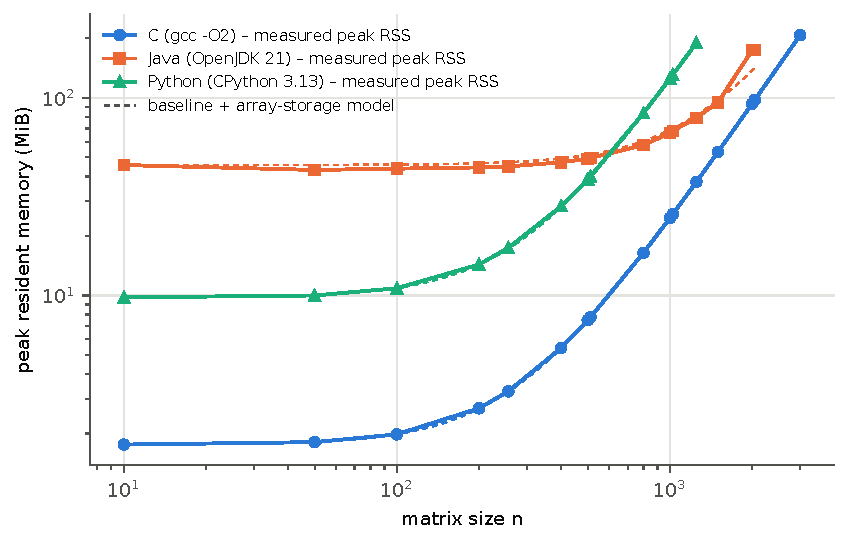
\includegraphics[width=0.82\linewidth]{../figures/fig3_memory.pdf}
\caption{Peak resident memory against $n$. Dashed lines: measured baseline of the smallest run plus the array-storage model ($24n^2$ B for C and Java, $120n^2$ B for Python).}
\label{fig:mem}
\end{figure}

C grows by $24.0$ bytes per $n^2$ (three $8$-byte matrices) on top of a $1.8$\,MiB baseline. Python grows by $120.9$ bytes
per $n^2$ ($5\times$ more) on top of $9.8$\,MiB, matching an $8$-byte pointer plus a $32$-byte float object per element
for three matrices. Java has the largest baseline ($45.7$\,MiB, the JVM itself) and grows by $\approx22$ bytes per $n^2$ up to
$n=1500$; at $n=2000$ and $2048$ it grows by $32$--$34$ bytes per $n^2$, i.e.\ about $32$\,MiB more than the three
arrays (not investigated; plausibly heap sizing by the garbage collector). The kernel's \texttt{ru\_maxrss}
(stored as a cross-check) is useless for small runs ($\approx 33$\,MiB even for C at $n=10$) because it counts the
parent driver's memory at process creation; this is why \texttt{VmHWM} was chosen as the primary metric.

\subsection{Feasible sizes and limits}
Table~\ref{tab:limits} separates the largest size that completed within the declared limits from the largest size
attempted. No run failed for memory. All failures are timeouts of a single multiplication at the $300$\,s limit; their
times are \emph{not} known, only that they exceeded $300$\,s.

\begin{table}[H]
\centering\small
\begin{tabular}{lrrl}
\toprule
Impl. & Largest feasible $n$ & Largest attempted $n$ & Outcome at largest attempted \\
\midrule
C & 3000 & 4096 & timeout ($>$300\,s per sample) \\
Java & 2048 & 3000 & timeout ($>$300\,s per sample) \\
Python & 1250 & 1500 & timeout ($>$300\,s per sample) \\
\bottomrule
\end{tabular}

\caption{Largest feasible and largest attempted size per implementation. The largest feasible size of every implementation was measured with only 2 repetitions.}
\label{tab:limits}
\end{table}

\subsection{Variability and warm-up}
Within a process, the relative IQR is mostly between $0.5$ and $20\,\%$ (Figure~\ref{fig:var}, left), with one outlier
of $36\,\%$ (C, $n=1250$); the median over all configurations is $4.8\,\%$. The first warm-up sample of Java is up to $1.3$--$1.6\times$ the steady median for some sizes
($n=50$, $400$, $500$) and about $1.0$ otherwise (right); with $3$ warm-up samples for the sizes below $1$\,s the
measured samples are in steady state. For the long runs (no warm-up) the first measured sample was within $10\,\%$ of the median (largest: $+10\,\%$, C at $n=2048$).

\begin{figure}[h]
\centering
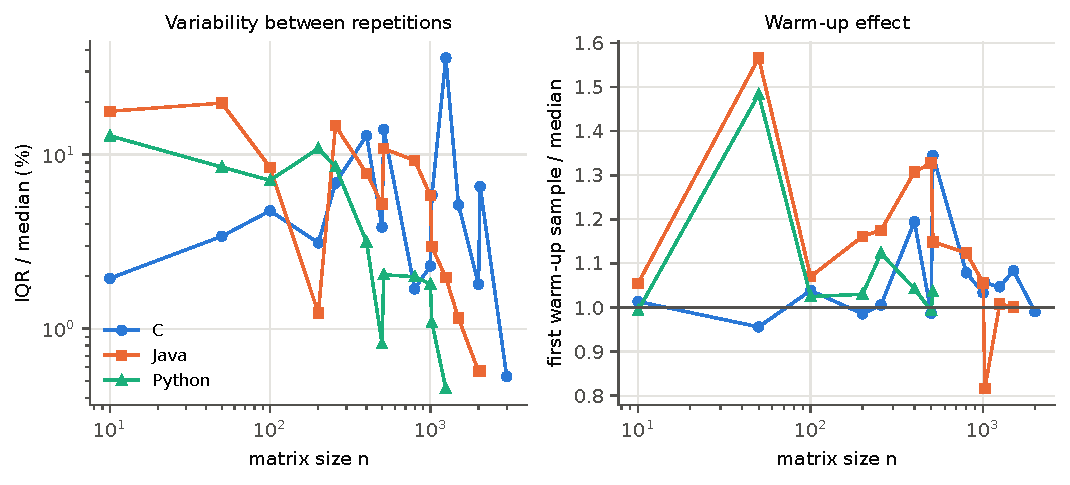
\includegraphics[width=0.95\linewidth]{../figures/fig4_variability_warmup.pdf}
\caption{Left: relative IQR of the measured samples within one process. Right: first warm-up sample divided by the median of the measured samples (only sizes with warm-up).}
\label{fig:var}
\end{figure}

\subsection{Supplementary experiments}

\paragraph{C optimisation level.}
\label{sec:cflags}
Table~\ref{tab:cflags} compares gcc optimisation levels. \texttt{-O0} is $2.2$--$3.7\times$ slower than \texttt{-O2}; \texttt{-O1},
\texttt{-O2}, \texttt{-O3} and \texttt{-O3 -march=native} are indistinguishable at $n=512$ and $n=1000$ ($\pm 6\,\%$) and differ by at
most $10\,\%$ at $n=1024$, which is within the between-process variability of Section~\ref{sec:procvar}. All variants produce the
same bits as \texttt{-O2}. The primary configuration \texttt{-O2} is therefore representative of the optimised builds for this
kernel; no vectorisation or loop interchange benefit was observed.

\begin{table}[H]
\centering\small
\begin{tabular}{lrrrc}
\toprule
Flags & $n{=}512$ & $n{=}1000$ & $n{=}1024$ & same bits as -O2 \\
\midrule
gcc -O0 & 638\,ms & 5.17\,s & 6.63\,s & yes \\
gcc -O1 & 299\,ms & 1.41\,s & 2.75\,s & yes \\
gcc -O2 & 292\,ms & 1.41\,s & 2.7\,s & yes \\
gcc -O3 & 267\,ms & 1.43\,s & 2.97\,s & yes \\
gcc -O3 -march=native & 278\,ms & 1.39\,s & 2.91\,s & yes \\
\bottomrule
\end{tabular}

\caption{C compiler options: median time per multiplication (10 repetitions at $n=512$, 5 otherwise).}
\label{tab:cflags}
\end{table}

\paragraph{Sizes around powers of two.}
\label{sec:pow2}
Table~\ref{tab:stride} and Figure~\ref{fig:pow2} show the time per multiply--add just below, at and above $2^9$ and
$2^{10}$. In C the time at $n=512$ and $n=1024$ is about $1.8$--$1.9\times$ that of the average of the neighbouring sizes
($n=512$: $2.41$ vs.\ $1.32$--$1.42$\,ns; $n=1024$: $3.04$ vs.\ $1.50$--$1.67$\,ns). The Java program with a flat array shows
the same spikes ($1.7$--$1.8\times$), whereas the Java program with \texttt{double[n][n]} shows none.

\begin{table}[H]
\centering\small
\begin{tabular}{rrrr}
\toprule
$n$ & C & Java \texttt{double[n][n]} & Java flat \texttt{double[]} \\
\midrule
496 & 1.417 & 1.631 & 1.411 \\
504 & 1.313 & 1.652 & 1.347 \\
512 & 2.410 & 1.576 & 2.325 \\
520 & 1.316 & 1.652 & 1.420 \\
1016 & 1.503 & 2.273 & 1.808 \\
1024 & 3.043 & 1.956 & 3.327 \\
1032 & 1.666 & 2.336 & 1.900 \\
\bottomrule
\end{tabular}

\caption{Median time per multiply--add (ns) around powers of two. Single process per cell.}
\label{tab:stride}
\end{table}

\begin{figure}[h]
\centering
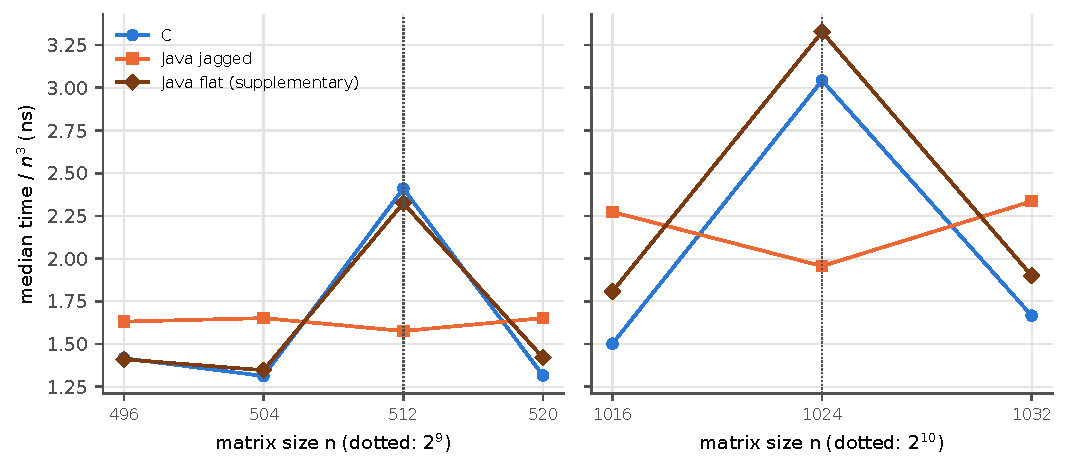
\includegraphics[width=0.92\linewidth]{../figures/fig7_powers_of_two.pdf}
\caption{Median time per multiply--add around $n=2^9$ (left) and $n=2^{10}$ (right).}
\label{fig:pow2}
\end{figure}

\paragraph{Java array layout.}
Table~\ref{tab:layout} and Figure~\ref{fig:layout} compare jagged and flat storage in Java against C. The flat
version is $1.07$--$1.49\times$ slower than C for $500\le n\le2000$, whereas the jagged version is $1.29$--$4.33\times$
slower; the jagged/flat ratio grows from $1.1$ at $n=500$--$1000$ to $1.7$--$2.9$ at $n\ge1250$. The $n=1250$ C
value has an IQR of $36\,\%$ and should be read with care.

\begin{table}[H]
\centering\small
\begin{tabular}{rrrrrr}
\toprule
$n$ & C & Java jagged & Java flat & jagged/C & flat/C \\
\midrule
500 & 154\,ms & 198\,ms & 169\,ms & 1.29 & 1.10 \\
1000 & 1.33\,s & 2.02\,s & 1.82\,s & 1.51 & 1.36 \\
1250 & 4.33\,s & 10.2\,s & 5.86\,s & 2.37 & 1.36 \\
1500 & 6.46\,s & 28\,s & 9.66\,s & 4.33 & 1.49 \\
2000 & 33.4\,s & 86.9\,s & 35.9\,s & 2.60 & 1.07 \\
\bottomrule
\end{tabular}

\caption{Median time per multiplication for C, Java with \texttt{double[n][n]} (jagged), and Java with a flat \texttt{double[]} (supplementary), and ratios.}
\label{tab:layout}
\end{table}

\begin{figure}[h]
\centering
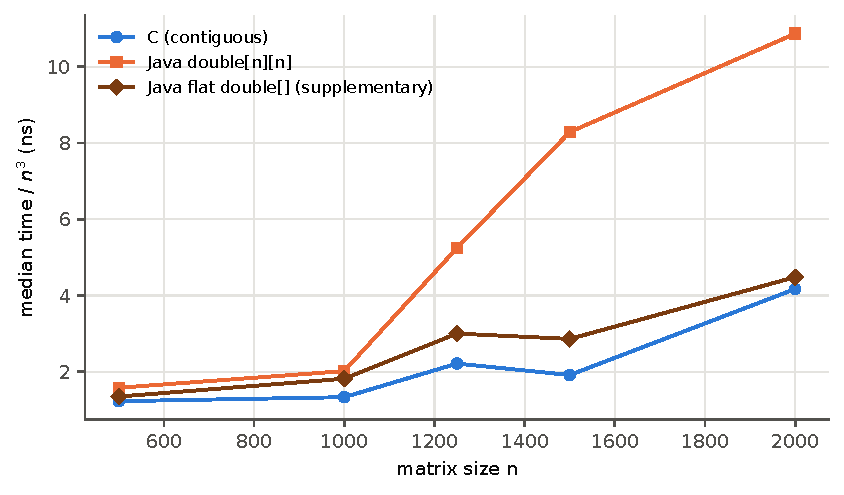
\includegraphics[width=0.82\linewidth]{../figures/fig8_java_layout.pdf}
\caption{Time per multiply--add for C and the two Java layouts.}
\label{fig:layout}
\end{figure}

\paragraph{Between-process variability.}
\label{sec:procvar}
Table~\ref{tab:procvar} reports the median time at $n=1024$ in six independent processes. For C the six medians
span $13\,\%$ of their median ($2.96$--$3.38$\,s), for Java $40\,\%$ ($2.10$--$3.21$\,s). Within each process the relative IQR
is $2$--$12\,\%$ for C and $3$--$28\,\%$ for Java (the min--max range of Java reaches $47\,\%$ of the median), so at this size the
timing is noisy both within and between processes. A single-process median at $n=1024$ is therefore uncertain by tens of
percent for Java, and differences of that size between C and Java at this $n$ cannot be resolved.

\begin{table}[H]
\centering\small
\begin{tabular}{lrr}
\toprule
Independent process & C & Java \\
\midrule
1 & 3.34\,s & 3.21\,s \\
2 & 3.27\,s & 2.1\,s \\
3 & 3.06\,s & 2.44\,s \\
4 & 2.96\,s & 2.75\,s \\
5 & 3.35\,s & 2.77\,s \\
6 & 3.38\,s & 3.08\,s \\
\textit{min} & 2.96\,s & 2.1\,s \\
\textit{median} & 3.3\,s & 2.76\,s \\
\textit{max} & 3.38\,s & 3.21\,s \\
range / median & 13\,\% & 40\,\% \\
\bottomrule
\end{tabular}

\caption{Median time per multiplication at $n=1024$ in six independent processes (process 1 is the main run).}
\label{tab:procvar}
\end{table}
